\documentclass{book}

\title{Quantum Information and Computing}
\newcommand{\booksubtitle}{A Textbook for Computer Science and Engineering Students}
\newcommand{\booklicense}{Creative Commons Zero 1.0 Universal}

\author{Yuan John Jiang}
% Author subtitle could be a university or a geographical location, for example
\newcommand{\authorsubtitle}{City, Country}

% Create convenient commands \booktitle and \bookauthor
\makeatletter
\newcommand{\booktitle}{\@title}
\newcommand{\bookauthor}{\@author}
\makeatother

% This utf8 declaration is not needed for versions of latex > 2018 but may
% be helpful for older software. Eventually it may not be worth keeping.
\usepackage[utf8]{inputenc}  
\usepackage{fix-cm}  % this package allows large \fontsize
\usepackage{tikz}    % this is for graphics. e.g. rectangle on title page
\usepackage{graphicx}
\usepackage{amsmath} % Used by equations

% The following dimensions specify 4.75" X 7.5" content on 6 3/8" by 9 1/4"
% paper. The paper width and height can be tweaked as required and the content
% should size to fit within the margins accordingly.
%
% The (inside) bindingoffset should be larger for books with more pages. Some
% standard recommended sizes are .375in minimum up to 1in for 600+ page books.
% Sizes .75in and .875in are also recommended roughly at 150 and 400 pages.
\usepackage[bindingoffset=0.625in,
            left=.5in, right=.5in,
            top=.8125in, bottom=.9375in,
            paperwidth=6.375in, paperheight=9.25in]{geometry}
% Here is an alternative geometry for reading on letter size paper:
% \usepackage[margin=.75in, paperwidth=8.5in, paperheight=11in]{geometry}

\renewcommand{\contentsname}{Table of Contents} % default is {Contents}
\usepackage{makeidx}
\makeindex % Initialize an index so we can add entries with \index

% The next few commands are for creating fake content to fill out the template.
% You should delete this (e.g.  everything up to, but not including,
% \begin{document}) after you insert your own content.
% Example content from Einstein's Meaning of Relativity.
% Public domain book: http://www.gutenberg.org/ebooks/36276
\newcommand{\fakeparagraph}{The theory of relativity experiences?}

\newcommand{\fakecontent}{
\fakeparagraph{}
\fakeparagraph{}

\fakeparagraph{}}

\newcommand{\fakesections}{
\fakecontent{}
\section{First Principles}\fakecontent{}
\subsection{Examples}\fakecontent{}
\subsection{Excessive Elaborations}\fakecontent{}
\subsection{Long Winded Conclusion}\fakecontent{}
\subsection{Exercises}\fakecontent{}
\section{Theory vs Practice}\fakecontent{}
\subsection{Examples}\fakecontent{}
\subsection{Excessive Elaborations}\fakecontent{}
\subsection{Long Winded Conclusion}\fakecontent{}
\subsection{Exercises}\fakecontent{}
\foreach \x in {A,B,C,D,E,F,G,H,I,J,K,L,M,N,O,P,Q,R,S,T,U,V,W,X,Y,Z}
    {\index{\x 1}\index{\x 2}}
}

% Content Starts Here
\begin{document}
\frontmatter

% No page numbers on the Frontispiece page
% \thispagestyle{empty}


% ---- Title Page ----
% current geometry will be restored after title page
\newgeometry{top=1.75in,bottom=.5in}
\begin{titlepage}
\begin{flushleft}

% Title
\textbf{\fontfamily{qcs}\fontsize{38}{50}\selectfont Quantum Information\\and Computing\\}

% Draw a line 4pt high
\par\noindent\rule{\textwidth}{4pt}\\

% Shaded box from left to right with Subtitle
% The text node is midway (centered).
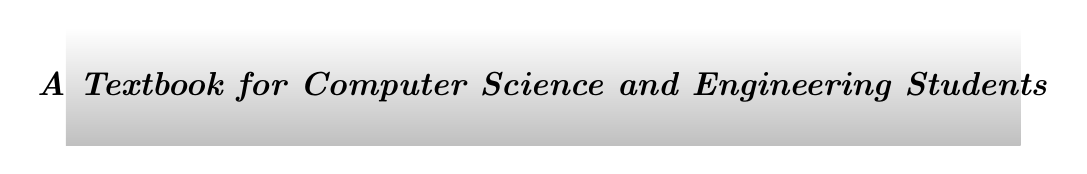
\begin{tikzpicture}
\shade[bottom color=lightgray,top color=white]
    (0,0) rectangle (\textwidth, 1.5)
    node[midway] {\textbf{\large \textit{\booksubtitle}}};
\end{tikzpicture}

% Edition Number
\begin{flushright}
\Large First Edition
\end{flushright}

\vspace{\fill}

% Author and Location
\textbf{\large \bookauthor}\\[3.5pt]
\textbf{\large \textit{\authorsubtitle}}

\vspace{\fill}

% Self Publishing Logo. Free to use: CC0 license.
% The source file is book.svg. If you change the svg, you must then convert
% it to pdf. There are many online and offline tools available to do that.
\begin{center}

\includegraphics{booksvg.pdf}\\[4pt]
\fontfamily{lmtt}\small{Self Publishers Worldwide\\
Seattle San Francisco New York\\
London Paris Rome Beijing Barcelona}
\end{center}

\end{flushleft}
\end{titlepage}
\restoregeometry
% ---- End of Title Page ----

% Do not show page numbers on colophon page
\thispagestyle{empty}

\begin{flushleft}
\vspace*{\fill}
This book was typeset using \LaTeX{} software.\\
\vspace{\fill}
Copyright \textcopyright{} \the\year{}  \bookauthor\\
License: \booklicense
\end{flushleft}

% A title page resets the page # to 1, but the second title page
% was actually page 3. So add two to page counter.
\addtocounter{page}{2}

% The asterisk excludes chapter from the table of contents.
\chapter*{Preface}
Quantum information and computing are hot topics, and there are many books around. But there is no book for computer science or engineering students who have not taken any courses on quantum physics. Of course, there are many popular science books and articles that explain quantum physics by drawing analogy to laymen observable things. But can one use the analogies of quantum superposition or entanglement to (IBM) QIS programming? This book is to bridge the gap between quantum physics and engineering so that information and computer sciences students can use their knowledge to implement or even develop quantum algorithms and protocols.

The difficulty of quantum physics lies in the wave behavior of particles. The focus of theoretical is how to solve the wave equations. And experimental physicists focus on how to control the waves. This book leaves out the details of the waves by labelling them with symbols e.g. "0" and "1". The symbols are what computer science and engineering students know how to work with. They are what the computer science data structure and algorithms, and Shannon information theory apply.

How to label waves with symbols is studied by encoding theory whose techniques have been studied by electrical engineering students. They are the bridge between physics in the analog world and information and computer sciences in the digital world.

% Three-level Table of Contents
\setcounter{tocdepth}{3}
\tableofcontents

\mainmatter

\chapter{Introduction}
The advantage of quantum computing lies in the possibility of parallel computing using a quantum system. Quantum information theory is mostly used in distributing encryption keys for telecommunication using quantum systems -- the so called quantum key distribution. The secrecy of quantum key exchange lies in the uncertainty of quantum measurement. If these statements are too abstract, read on.

\section{The Advantage of Parallel Exploration}
\subsection{The Maze Problem}
Maze problems are hard. That's because there are too many paths to explore from the entrance to the exit. Computer scientists have long known parallel computing is the way to speed up finding solutions to such problems.

\begin{figure}[ht]
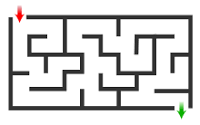
\includegraphics[width=6cm]{maze.png}
\caption{Maze}
\label{Maze}
\end{figure}

For a physicist, this experiment is the fast approach to a solution: run water into the entrance. If we see water out of the exit, we know the maze problem has at least one solution. But do we know whether there are more than one good paths or how many good paths there are? We can refine the experiment: run several water drops into the entrance. Of course, these are not the solution to the final maze problem, but we can keep on adding water tricks toward a solution.
Of course the solutions to such hard problems are to explore all the paths in parallel. Let’s look at how a physicist would use parallel exploration to solve the maze problems.

For the simplest case – we want to know if there is any good path at all. We can put water into the entrance. If there is any water coming out of the exit, we know the answer is positive. Adding complexity to the problem, we want to know how many good paths there are? Again, we can play the water trick. Let’s put several water drops into the entrance and see how many drops will come out. Until now, we don't have the solution to the final maze problem, but we can keep on adding water tricks toward a solution.

Playing with water tricks is exactly the idea behind quantum computers. Quantum physics tells us every particle possesses both wave behavior and particle behavior. The wave behavior is like the watery behavior and allows the wave to spread and propagate through out all possible paths. The particle behavior gives use the “drop” behavior and allows the particle to reveal the properties, e.g. the length, of the individual paths.
\subsection{Waves}
We use electromagnetic waves every day. We get Wi-Fi or cellphone signals even when we move around the house or on the streets because the waves can spread and explore unlimited paths to reach us. We can contain electromagnetic waves in boxes. Microwave ovens are examples. We can also optical fibers, co-axile cables and waveguides to channel electromagnetic waves in one dimension along the cable lengths.

All matters, e.g. electrons, are waves in nature. If electrons were not waves, they would collapse to the positively charged nucleus and result in atoms of zero sizes, and we would have not seen the world as we have.

\subsection{Particles}
A particle is the smallest "drop" of matter. But "the smallest" by what measure? That is a critical question we should ask. By the amount of energy, a photon is the smallest drop of an electromagnetic wave. An electron is the smallest drop if measured by both mass and electric charge.

The waves and matters we see or use everyday contain too many particles, and we only see the average effects of the waves and matters. If we have two beams of lights, one is yellow and the other blue, merged into one, what do we see? We see a beam of green light. But if we lower the emissions from each of the lights to one photon at a time, we will see either a yellow or blue photon -- we don't see a green photon. 

The sound from a guitar string play note E is different in our ears from that played on a violin. That is because the sound from each is composed by many harmonics, an octave apart from each other. The average or combined effects from the strings of different instruments is different. If our ears were sensitive enough to hear individual phonons -- the smallest drops of sound -- we would hear sound of pure harmonics.

Of course making such single particle, photon or phonon, generators or detectors has been the very challenge to physicists in their effort to make quantum computing and communication.

\subsection{State and superposition}
From a wave's perspective, we see particles in it. From a particle's perspective, we can imagine it rides on a wave like a surfer following the trajectry defined by the wave. State is a quantum physics term referring to the wave that a particle rides on. Physicists use the wavefunction $\psi$ of the wave to note the state $|\psi>$ - the so called "ket" notation. But throughout this book, we use the labels e.g. "0" and "1" of the waves to note the states as $|0>$ and $|1>$. 

Can a particle be in two waves? Yes, it can. The two waves may be viewed as two by one measurement but are one by another measurement. 

\chapter{Qubits for computing}
\chapter{Qubits for communication}
\chapter{Bibliography}
\chapter{General Tendencies}

\backmatter
\addcontentsline{toc}{chapter}{Index}
\printindex
\end{document}